\documentclass[10pt]{article}

\usepackage{proceed2e}
\usepackage{myuaistyle}

\setlength{\abovedisplayskip}{0pt} 
\setlength{\belowdisplayskip}{0pt} 
\setlength{\abovedisplayshortskip}{0pt}
\setlength{\belowdisplayshortskip}{0pt}

% Figures directory
\graphicspath{{./figures/}}

\newcommand{\contmax}{\mathrm{max}}
\newcommand{\casemax}{\mathrm{casemax}}
\newcommand{\casemin}{\mathrm{casemin}}

\begin{document}

\title{Closed-form Solutions to a Subclass of Continuous Stochastic Games via Symbolic Dynamic Programming}


\author{}

% The author names and affiliations should appear only in the accepted paper.
%
%\author{ {\bf Harry Q.~Bovik\thanks{Footnote for author to give an
%alternate address.}} \\
%Computer Science Dept. \\
%Cranberry University\\
%Pittsburgh, PA 15213 \\
%\And
%{\bf Coauthor}  \\
%Affiliation          \\
%Address \\
%\And
%{\bf Coauthor}   \\
%Affiliation \\
%Address    \\
%(if needed)\\
%}


\maketitle
While convex losses for binary classification are attractive due to
the existence of numerous (provably) efficient methods for finding
their global optima, they are sensitive to outliers.  On the other
hand, while the non-convex 0--1 loss is robust to outliers, it is
NP-hard to optimize and thus rarely directly optimized in practice.
In this paper, however, we do just that: we explore a variety of
practical methods for direct (approximate) optimization of the 0--1
loss based on branch and bound search, combinatorial search, and
coordinate descent on smooth, differentiable relaxations of 0--1 loss.
Empirically, we compare our proposed algorithms to logistic
regression, SVM, and the Bayes point machine showing that the proposed
0--1 loss optimization algorithms perform at least as well and offer a
clear advantage in the presence of outliers.  To this end, we believe
this work reiterates the importance of 0--1 loss and its robustness
properties while challenging the notion that it is difficult to
directly optimize.

\section{Introduction}
%-----------------------------------------------------------------------------
%  What is the problem
%  Why is it interesting
%  What are your contributions
%  What is the outline
%-----------------------------------------------------------------------------

Modelling sequential competitive interactions between agents \\has 
important applications within economics and decision making. 
Stochastic games \cite{Shapley_PotNAoS_1953} provide framework 
a to model sequential interactions between multiple
non-cooperative \\agents. Zero-sum stochastic games stipulate that the
participating agents have diametrically opposing goals. 
Littman \cite{Littman_ICML_1994} presented a multiagent reinforcement
learning solution to discrete state zero-sum stochastic games. 
Closed form solutions for the continuous state case, however, 
remain unknown. Continuous state zero-sum stochastic games provide
a convenient framework with which to model many important financial
and economic domains, such as option valuation on derivative markets.

In this paper we present a novel technique to calculate a closed-form
solution to a subclass of continuous state zero-sum stochastic games. 
We show that by using symbolic dynamic programming we can calculate
closed-form solutions for arbitrary horizons.

We begin by presenting Markov Decision Processes (MDPs) and value
iteration \cite{Bellman_1957}, a commonly used dynamic programming
solution. We then describe both discrete and continuous stochastic 
games, game theoretic generalisations of the MDP framework. 
Following this we show how Symbolic Dynamic Programming (SDP) 
\cite{Boutilier_IJCAI_2001} can be used to calculate exact solutions
to a particular subclass of continuous zero-sum stochastic games. 
Finally, we present an empirical evaluation of our novel technique on 
an American option quitting game.
\section{Markov Decision Processes}
\label{sec:mdp}

A Markov Decision Process (MDP) \cite{Howard_1960} is defined by the tuple
$ \left\langle S, A, T, R, h, \gamma \right\rangle$. $S$ and $A$ 
specify a finite set of states and actions, respectively.
$T$ is a transition function $T : S \times A \rightarrow S$ which 
defines the effect of an action on the state. $R$ is the
reward function $R : S \times A \rightarrow \mathbb{R}$ which 
encodes the preferences of the agent. The horizon $h$ represents the 
number of decision steps until termination and the discount factor $\gamma$ 
is used to discount future rewards. In general, an agent's objective is 
to find a policy, $\pi : S \rightarrow A$, which maximises the expected 
sum of discounted rewards over horizon $h$.

Value iteration \cite{Bellman_1957} is a general dynamic programming 
algorithm used solve MDPs. For each horizon $h$, two functions form 
the basis of the algorithm: $V^{h}(s)$, the value of state $s$, and 
$Q^{h}(s, a)$, the value of taking action $a$ in state $s$. The two 
functions satisfy the following recursive relationship:
\begin{align}
  Q^{h}(s, a) &= R(s, a) + \gamma \sum_{s' \in S} T(s, a, s') V^{h-1}(s') \\
  V^{h}(s) &= \max_{a \in A} Q^{h}(s, a).
\end{align}

The algorithm is executed by first initialising $V^{0}$  to $R(s, a)$. 
Then for each $h$, the value function for $V^{h}(s)$ is calculated from $V^{h-1}(s)$
until the intended $h$-stage-to-go value function is computed.
Value iteration converges linearly in the number of iterations to the true
values of $Q(s, a)$ and $V(s)$ \cite{Bertsekas_1987}.

MDPs can be used to model multiagent systems under the assumption 
that other agents are part of the environment and have fixed behaviour. 
As a result, they ignore the difference between responsive agents and 
a passive environment \cite{Hu_ICML_1998}. In the next section we 
present a game theoretic framework which generalises MDPs to 
situations with two or more agents.
\section{Zero-sum Discrete Stochastic Games}
\label{sec:dsg}
Discrete state stochastic games (DSGs) are formally defined by the tuple
$ \left\langle S, A_{1}, \ldots, A_{n}, T, R_{1}, \ldots, R_{n}, h, \gamma\right\rangle$.
$S$ is a set of discrete states and $A_i$ is the action set available to agent 
$i$. T is a transition function $T : S \times A_1 \times \ldots \times A_n \rightarrow \Delta(S)$, 
where $\Delta(S)$ is the set of probability distributions over the state space $S$. 
The reward function $R_i : S \times A_1 \times \ldots \times A_n \rightarrow \mathbb{R}$ 
encodes the individual preferences of agent $i$. The horizon $h$ represents the 
number of decision steps until termination and the discount factor $\gamma \in [0, 1)$ 
is used to discount future rewards. In general, an agent's objective is 
to find a policy, $\pi_i : S \rightarrow \sigma_i(A_i)$ which maximises the expected 
sum of discounted rewards over horizon $h$. Here $\sigma_i(A_i)$ specifies
probability distributions over action set $A_i$. The optimal policy in a 
DSG may be stochastic, that is, it may define a mixed strategy for each state. 

%The goal of each agent in a stochastic game is to maximise its expected 
%discounted future rewards.

%Two agent zero-sum DSGs impose a condition on the reward structure 
%of the game whereby the goals of an agent and its opponent are diametrically
%opposed to one another. Under this restriction the reward structure can 
%be represented by a single reward function. The opponent's
%reward function is simply the opposite of the agent's. 
%Within this game 
%each agent attempts to maximise its expected discounted future rewards 
%in the minimax sense. Since the reward structure is zero-sum it is sufficient to view the 
%opponent as acting to minimise the agent's return.

Zero-sum DSGs are a type of DSG involving two agents with diametrically
opposing goals. Under these conditions the reward structure for the 
game can be represented by a single reward function since an agents
reward function is simply the opposite of their opponent's. The objective
of each agent is to maximise its expected discounted future rewards 
in the minimax sense. That is, each agent views its opponent as
acting to minimise the agent's reward. Zero-sum DSGs can be solved 
using a technique analogous to value iteration for MDPs \cite{Littman_ICML_1994}. 
The value function, $V^{h}(s)$, in this setting can be defined as:

\vspace{-7.5mm}
{\small

%\abovedisplayskip=0pt
\belowdisplayskip=0pt
%\allowdisplaybreaks
\begin{multline}
\label{eq:dsgvfunc}
  V^{h}(s) = \\
  \max_{m \in \sigma_1(A_1)} \hspace{2pt} \min_{o \in \sigma_2(A_2)} \sum_{a_1 \in A_1} \sum_{a_2 \in A_2} Q^{h}(s, a_1, a_2) \cdot m_{a_{1}} \cdot o_{a_{2}}
\end{multline}
}%

where $m$ and $o$ are mixed strategies from $\sigma_1(A_1)$ and
$\sigma_2(A_2)$, respectively. $Q^{h}(s, a_1, a_2)$, the quality of taking action $a_1$ against action $a_2$ in state $s$,
is given by:

\vspace{-6.5mm}
{\small 
%\abovedisplayskip=0pt
\belowdisplayskip=0pt
\begin{multline}
\label{eq:dsgdiscqfunc}
  Q^{h}(s, a_1, a_2) = R(s, a_1, a_2) + \\
  \gamma \cdot \sum_{s' \in S} T(s, a_1, a_2, s') \cdot V^{h-1}(s').
\end{multline}
}%

%It is well known that Equation \eqref{eq:dsgvfunc} can be further simplified to:
Equation \eqref{eq:dsgvfunc} can be further simplified by noting that
since the $\text{min}$ operation is ``inside'' the $\text{max}$, the minimum is achieved
for a deterministic action choice. This observation leads to the following
form:

\vspace{-6.5mm}
{\small 
%\abovedisplayshortskip =100pt
%\belowdisplayshortskip =100pt
\begin{equation}
\label{eq:dsgvfunccompact}
  V^{h}(s) = \max_{m \in \sigma_1(A_1)} \min_{a_2 \in A_2} \sum_{a_1 \in A_1} Q^{h}(s, a_1, a_2) \cdot m_{a_1}.
\end{equation}
}%
\vspace{-6.5mm}

Together Equations \eqref{eq:dsgdiscqfunc} and \eqref{eq:dsgvfunccompact}
define a recursive method to calculate the optimal solution to zero-sum
DSGs. The policy for the opponent can be calculated by applying symmetric
reasoning and the Minimax theorem \cite{Neumann_MA_1928}. 

\subsection{Solution Techniques}
\label{subsec:dsgsolution}

Zero-sum DSGs can be solved via discrete linear optimisation. The value
function in Equation \eqref{eq:dsgvfunccompact} can be reformulated as a linear
program through the following steps:

\begin{enumerate}
  \item Define $V^h(s)$ to be the value of the inner minimisation term in
            Equation \eqref{eq:dsgvfunccompact}. This leads to the following linear program for a known state $s$:
{\small
\abovedisplayskip=10pt
\belowdisplayskip=0pt 
\begin{subequations}
\begin{align}
&\text{maximise}   \  V^{h}(s) \nonumber \\
&\text{subject to}   \nonumber \\
&\  V^{h}(s) = \min_{a_2 \in A_2} \sum_{a_1 \in A_1} Q^{h}(s, a_1, a_2) \cdot m_{a_{1}} \label{eq:dsglpconstraint1} \\
                          &\  \sum_{a_{1} \in A_1} m_{a_{1}} = 1 ; \  m_{a_{1}} \geq 0 \qquad \forall a_{1} \in A_1 \nonumber
\end{align}
\end{subequations}
}%

  \item Replace the equality (=) in constraint \eqref{eq:dsglpconstraint1} with
  $\leq$ by observing that the maximisation of $V^{h}(s)$
  effectively pushes the $\leq$ condition to the = case. This gives: 
{\small 
\abovedisplayskip=8pt
\belowdisplayskip=0pt
\begin{subequations}
\begin{align}
&\text{maximise}   \  V^{h}(s) \nonumber \\
&\text{subject to}   \nonumber \\
&\  V^{h}(s) \leq \min_{a_2 \in A_2} \sum_{a_1 \in A_1} Q^{h}(s, a_1, a_2) \cdot m_{a_{1}} \label{eq:dsglpconstraint2} \\
                          &\  \sum_{a_{1} \in A_1} m_{a_{1}} = 1 ; \  m_{a_{1}} \geq 0 \qquad \forall a_{1} \in A_1 \nonumber
\end{align}
\end{subequations}
}%
  
  \item Remove the minimisation operator in constraint \eqref{eq:dsglpconstraint2}
            by noting that the minimum of a set is less than or equal to the minimum of all elements in the set.
            This leads to the final form of the discrete linear optimisation problem:
{\small 
\abovedisplayskip=8pt
\belowdisplayskip=0pt
\begin{align*}
&\text{maximise}   \  V^{h}(s) \nonumber \\
&\text{subject to}   \nonumber \\
&\  V^{h}(s) \leq \sum_{a_1 \in A_1} Q^{h}(s, a_1, a_2) \cdot m_{a_{1}} \ \forall a_2 \in A_2\\
                          &\  \sum_{a_{1} \in A_1} m_{a_{1}} = 1 ; \  m_{a_{1}} \geq 0 \qquad \forall a_{1} \in A_1 \nonumber
\end{align*}
}%
\end{enumerate}

We can now use existing linear programming solvers to compute the optimal
solution to this linear program for each $s \in S$ at a given horizon $h$.

The linear program used to solve zero-sum DSGs cannot be used once
the state is continuous since there are infinitely many states. The key 
innovation of this paper is in showing that continuous state zero-sum
games can still be solved through the use of symbolic dynamic programming.
\section{Zero-sum Continuous Stochastic Games}
\label{sec:csg}

Continuous state stochastic games (CSGs) are formally defined by the tuple
$ \left\langle \vec{x}, A_{1}, \ldots, A_{n}, T, R_{1}, \ldots, R_{n}, h, \gamma  \right\rangle$.
In CSGs states are represented by vectors of continuous variables, $\vec{x} = \left(x_1, \ldots, x_m \right)$, 
where $x_i \in \mathbb{R}$. The other components of the tuple are as 
previously defined in Section~\ref{sec:dsg}.

Zero-sum CSGs impose the same restrictions on the number of agents
and the reward structure as their discrete state counterparts. 

The optimal solution to zero-sum CSGs can be calculated via the following 
recursive functions:

{\small
\abovedisplayskip=0pt
\belowdisplayskip=0pt
\begin{align}
\label{eq:csgdiscqfunc}
  Q^{h}(\vec{x}, a_1, a_2) &= R(\vec{x}, a_1, a_2) \quad + \nonumber \\
  & \qquad  \gamma \cdot \int T(\vec{x}, a_1, a_2, \vec{x}') \cdot V^{h-1}(\vec{x}')\ d\vec{x}'
\end{align}
}%

{\small 
\abovedisplayskip=0pt
\belowdisplayskip=0pt
\begin{align}
\label{eq:csgvfunccompact}
  V^{h}(\vec{x}) = \max_{m \in \sigma(A_1)} \min_{a_2 \in A_2} \sum_{a_1 \in A_1} Q^{h}(\vec{x}, a_1, a_2) \cdot m_{a_{1}}
\end{align}
}%

We can derive Equation \eqref{eq:csgdiscqfunc} from Equation \eqref{eq:dsgdiscqfunc}
by replacing $s$, $s'$ and the $\sum$ operator with their continuous
state counterparts, $\vec{x}$, $\vec{x}'$ and $\int$, respectively. Equation~\eqref{eq:csgvfunccompact}
is simply Equation~\eqref{eq:dsgvfunccompact} restated.

\subsection{Solution Techniques}

Zero-sum CSGs can be solved using a technique analogous to that 
presented in Section \ref{subsec:dsgsolution}. Namely, the value function in Equation
\eqref{eq:csgvfunccompact} can be reformulated as the following continuous 
optimisation problem:

{\small 
\abovedisplayskip=0pt
\belowdisplayskip=0pt
\begin{subequations}
\begin{align}
&\text{maximise}   \  V^{h}(\vec{x}) \nonumber \\
&\text{subject to}   \nonumber \\
&\   V^{h}(\vec{x}) \leq \sum_{a_1 \in A_1} Q^{h}(\vec{x}, a_1, a_2) \cdot m_{a_{1}} \   \forall a_2 \in A_2 \label{eq:bilinearconstraint} \\
                          &\  \sum_{a_{1} \in A_1} m_{a_{1}} = 1 ; \  m_{a_{1}} \geq 0 \qquad \forall a_{1} \in A_1 \nonumber
\end{align}
\end{subequations}
}%

This optimisation problem cannot be easily solved using existing techniques
due to two factors: (1) there are infinitely many states in $\vec{x}$; and
(2) constraint \eqref{eq:bilinearconstraint} is nonlinear in $\vec{x}$ and 
$m_{a_{1}}$ for general representations of {\small $Q^{h}(\vec{x}, a_1, a_2)$}. 
To further illustrate the second limitation consider {\small $Q^{h}(\vec{x}, a_1, a_2)$} in the 
form of a linear function in $x$, for some $a_1$ and $a_2$:

{\small 
\abovedisplayskip=0pt
\belowdisplayskip=0pt
\begin{align}
Q^{h}(\vec{x}, a_1, a_2) = \sum_{j} c_j \cdot x_j \label{eq:linqfunc}
\end{align}
}%

Substituting Equation \eqref{eq:linqfunc} into constraint \eqref{eq:bilinearconstraint}
yields:

{\small 
\abovedisplayskip=0pt
\belowdisplayskip=0pt
\begin{align}
V^{h}(\vec{x}) \leq \sum_{a_1 \in A_1} m_{a_{1}} \sum_{j} c_j \cdot x_j \qquad \forall a_2 \in A_2. \label{eq:linqfuncresult}
\end{align}
}%

It is clear from Equation \eqref{eq:linqfuncresult} that a linear representation
of {\small $Q^{h}(\vec{x}, a_1, a_2)$} leads to a nonlinear constraint
where $m_{a_{1}}$ must be optimal with respect to the free variable
$\vec{x}$. This results in a parameterised nonlinear program, whose optimal solutions are known to be
NP-hard \cite{Bennett_COA_1993,Petrik_JoMLR_2011}.

At this point we present the first key insight of this paper: we can 
transform constraint~\eqref{eq:bilinearconstraint} from a 
parameterised nonlinear constraint to a piecewise linear constraint by 
imposing the following restrictions: (1) restricting the reward function, 
{\small $R(\vec{x}, a_1, a_2)$}, to piecewise constant functions; and 
(2) restricting the transition function, 
{\small $T(\vec{x}, a_1, a_2, \vec{x}')$}, to piecewise linear functions. 
As a result, {\small $V^{h}(\vec{x})$} and 
{\small $Q^{h}(\vec{x}, a_1, a_2)$} will be piecewise constant functions, thereby
guaranteeing a tractable solution to constraint~\eqref{eq:bilinearconstraint}.

One key challenge still remains, namely, dealing with the infinitely
many states in $\vec{x}$. We know that the {\small $V^{h}(\vec{x})$} and 
{\small $Q^{h}(\vec{x}, a_1, a_2)$} functions have structure, but are unable to derive
them. Furthermore, given known structures for {\small $V^{h}(\vec{x})$} and 
{\small $Q^{h}(\vec{x}, a_1, a_2)$} we must determine the restrictions that
guarantee a tractable solution. The SDP framework in conjunction with its
closed-form operations provide answers to both of these concerns.

%------------------------------------------------------------------------------

%In spite of this insight, two questions still remain: (1) how do we 
%determine the structure of {\small $V^{h}(\vec{x})$} and (2) if we 
%know the structure of {\small $V^{h}(\vec{x})$}, how do we solve the 
%continuous optimisation problem ? Symbolic dynamic programming 
%allows us to derive the structure of {\small $V^{h}(\vec{x})$} and 
%bypass solving the continuous optimisation problem by implementing 
%Equations~\eqref{eq:csgdiscqfunc} and ~\eqref{eq:csgvfunccompact} 
%directly.

In the next section we show that zero-sum CSGs, with the 
aforementioned restrictions, can be solved optimally for arbitrary 
horizons using symbolic dynamic programming.
\section{Symbolic Dynamic Programming}
\label{sec:sdp}

Symbolic dynamic programming (SDP) \cite{Boutilier_IJCAI_2001} is 
the process of performing dynamic programming via symbolic 
manipulation. In the following sections we present a brief overview
of SDP and the data structures used to perform operations.

\subsection{Case Representation}

Symbolic dynamic programming assumes that all continuous symbolic 
functions can be represented in case form \cite{Boutilier_IJCAI_2001}.

\begin{equation}
  f = 
    \begin{cases}
      \phi_1: & f_1 \\ 
      \vdots & \vdots\\ 
      \phi_k: & f_k \\ 
    \end{cases} \nonumber
\end{equation}

$\phi_i$ are logical formulae defined over the state $\vec{x}$ 
and can include arbitrary logical combinations of boolean variables and 
linear inequalities over continuous variables. Each $\phi_i$ will be 
disjoint from the other $\phi_j$ ($j \neq i$) and may not 
exhaustively cover the state space. Hence, \emph{f} may only be a 
partial function. The $f_i$ may be either linear or quadratic 
in the continuous parameters. Operations on $f_i$ preserve the 
continuous nature of the function $f$.
 
%Symbolic dynamic programming assumes that all symbolic functions 
%can be represented in case form \cite{Boutilier_IJCAI_2001}, that is,
%
%\begin{equation}
  %f = 
    %\begin{cases}
      %\phi_1: & f_1 \\ 
      %\vdots & \vdots\\ 
      %\phi_k: & f_k \\ 
    %\end{cases} \nonumber
%\end{equation}
%
%where $\phi_i$ are logical formulae defined over the state $\vec{x}$ 
%that can include arbitrary logical ($\land, \lor, \neg$) combinations of 
%boolean variables and linear inequalities ($\geq, >, \leq, <$) over 
%continuous variables. The function \emph{f} is required to be continuous.
%
%Each $\phi_i$ will be disjoint from the other $\phi_j$ ($j \neq i$); 
%however the $\phi_i$ may not exhaustively cover the state space, hence
%\emph{f} may only be a partial function and may be undefined for 
%some variable assignments. The $f_i$ may be either linear or quadratic 
%in the continuous parameters according to the same restrictions as for 
%$R(\vec{x}, a, \vec{y})$.

\subsection{Case Operations}

Unary operations on a case statement \emph{f}, such as scalar 
multiplication $c \cdot f$ where $ c \in \mathbb{R} $ or negation $-f$,
are applied to each $f_i$ ($1 \leq i \leq k$). 

Binary operations on two case statements are executed in two stages.
Firstly, the cross-product of the logical partitions of each case statement 
is taken, producing paired partitions. Finally, the binary operation 
is applied to the resulting paired partitions. The ``cross-sum'' $\oplus$
operation can be performed on two cases in the following manner:

\begin{center}
  \begin{tabular}{r c c c l}
  &
    $\begin{cases}
        \phi_1: \hspace{-1mm} & \hspace{-1mm} f_1  \\ 
        \phi_2: \hspace{-1mm} & \hspace{-1mm} f_2  \\ 
    \end{cases}$
  $,$
  &
  \hspace{-4mm}
    $\begin{cases}
        \psi_1: \hspace{-1mm} & \hspace{-1mm} g_1  \\ 
        \psi_2: \hspace{-1mm} & \hspace{-1mm} g_2  \\ 
    \end{cases}$
  &
  \hspace{-4mm} 
  $ = $
  &
  \hspace{-4mm}
    $\begin{cases}
      \psi_1 \wedge \psi_1: & f_1 + g_1 \\
      \psi_1 \wedge \psi_2: & f_1 + g_2 \\
      \psi_2 \wedge \psi_1: & f_2 + g_1 \\
      \psi_2 \wedge \psi_2: & f_2 + g_2  \\
    \end{cases}$
  \end{tabular}
\end{center}

``cross-subtraction''  $\ominus$ and ``cross-multiplication'' $\otimes$
are defined in a similar manner but with the addition operator replaced
by the subtraction and multiplication operators, respectively.
Some partitions resulting from case operators may be inconsistent and 
are thus removed. 

Maximisation over cases, known as $\casemax$, is defined as:
\begin{center}
  \begin{tabular}{r c c c l}
  &
  \hspace{-7mm} $\casemax \Bigg(
    \begin{cases}
        \phi_1: \hspace{-1mm} & \hspace{-1mm} f_1 \\ 
        \phi_2: \hspace{-1mm} & \hspace{-1mm} f_2 \\ 
    \end{cases}$
  $,$
  &
  \hspace{-4mm}
    $\begin{cases}
        \psi_1: \hspace{-1mm} & \hspace{-1mm} g_1 \\ 
        \psi_2: \hspace{-1mm} & \hspace{-1mm} g_2 \\ 
    \end{cases} \Bigg)$
  &
  \hspace{-4mm} 
  $ = $
  &
  \hspace{-4mm}
    $\begin{cases}
      \phi_1 \wedge \psi_1 \wedge f_1 > g_1    : & \hspace{-2mm} f_1 \\ 
      \phi_1 \wedge \psi_1 \wedge f_1 \leq g_1 : & \hspace{-2mm} g_1 \\ 
      \phi_1 \wedge \psi_2 \wedge f_1 > g_2    : & \hspace{-2mm} f_1 \\ 
      \phi_1 \wedge \psi_2 \wedge f_1 \leq g_2 : & \hspace{-2mm} g_2 \\ 
      \vdots & \vdots
    \end{cases}$
  \end{tabular}
\end{center}

$\casemax$ preserves the linearity of its inputs. If the $f_i$ or 
$g_i$ are quadratic then the expressions $f_i > g_i$ or 
$f_i \leq g_i$ will be at most univariate quadratic and any such 
constraint can be linearised into a combination of at most two linear 
inequalities by completing the square.

\subsection{Extended Algebraic Decision Diagrams for Case Statements}

Case statements and their operations are implemented using Extended 
Algebraic Decision Diagrams (XADDs) \cite{Sanner_UAI_2011}.
XADDs provide a compact data structure with which to maintain
compact forms of $Q(\vec{x}, a_1, a_2)$ and $V(\vec{x})$. 
XADDs also permit the use of linear constraint feasibility checkers to 
prune unreachable paths in the XADD.

\subsection{SDP Solution Continuous Stochastic Games}

Symbolic dynamic programming can be used to find a closed-form
solution to a continuous stochastic game over an arbitrary horizon.

%%%%%%%%%%%%%%%%%%%%%%%%%%%%%%%%%
\incmargin{.5em}
\linesnumbered
\begin{algorithm}[H]
  \vspace{-.5mm}
  \dontprintsemicolon
  \SetKwFunction{regress}{Regress}
  
  \Begin{
    $V^0:=0, h:=0$\;
    \While{$h < H$}{
      $h:=h+1$\;
      
      $Q^h := \int V^{h-1} \otimes T(\vec{x}', \vec{x}, a_1, a_2) d_{\vec{x}'}$\;
      $Q^h := R(\vec{x}, a_1, a_2) \oplus (\gamma \otimes Q^h)$\;
      
      %$V^{h} := \casemax_{\pi_{a_1} \in \sigma(A_1)} \, Q_a^{h}$ $,$ \;      
      
      %\ForEach {$a(\vec{y}) \in A$}{
        %$Q_a^{h}(\vec{y})\,:=\,$\regress{$V^{h-1},a,\vec{y}$}\;
        %$Q_a^{h} := \casemin_{a_2 \in A_2} \, Q_a^{h}(\vec{y})$ $\,$\;
        %$V^{h} := \casemax_{\pi_{a_1} \in \sigma(A_1)} \, Q_a^{h}$ $,$ \;        
      %}
      
      \If{$V^h = V^{h-1}$} {
        break 
        $\,$ \emph{// Terminate if early convergence}\;
      }
    }    
    \Return{$(V^h)$} \;
  }
  \caption{
    \footnotesize \texttt{VI}(CSG, $H$) $\longrightarrow$ $(V^h)$ 
    \label{alg:vi}
  }
  \vspace{-1mm}
\end{algorithm}
\decmargin{.5em}
%%%%%%%%%%%%%%%%%%%%%%%%%%%%%%%%%

%%%%%%%%%%%%%%%%%%%%%%%%%%%%%%%%%
\incmargin{.5em}
\linesnumbered
\begin{algorithm}[H]
  \vspace{-.5mm}
  \dontprintsemicolon
  \SetKwFunction{remapWithPrimes}{Prime}
  %\SetKwFunction{sumout}{sumout}

  \Begin{
    $Q=$ \remapWithPrimes{$V$} $\,$ \emph{// All $ x_i \to x_i'$} \;
    \emph{// Continuous regression marginal integration}\\
    \For {all $x'_j$ in $Q$}{
      $Q := \int Q \otimes P(x_j'|\vec{x}, a_1, a_2) d_{x'_j}$\;
    }
    \Return{$R(\vec{x}, a_1, a_2) \oplus (\gamma \otimes Q)$} \;
  }
  \caption{
    \label{alg:regress}
    \footnotesize \texttt{Regress}($V, a_1, a_2$) $\longrightarrow$ $Q$   
  }
  \vspace{-1mm}
\end{algorithm}
\decmargin{.5em}
%%%%%%%%%%%%%%%%%%%%%%%%%%%%%%%%%
\section{Empirical Results}
\label{sec:results}

In this section we evaluate our novel SDP solution technique for zero-sum CSGs 
on three continuous domains\footnote{\fontsize{8pt}{10pt}\selectfont All of the source code can be found online at 
\texttt{http://code.google.com/p/xadd-inference}.}: 
(1) continuous stochastic matching pennies; (2) 
binary option stochastic game; and (3) robust energy production. The results represent
the first known exact solutions to these domains. 

\subsection{Continuous Stochastic Matching Pennies}

Matching pennies is a well known zero-sum game with a 
mixed strategy Nash Equilibrium \cite{Osborne_2004}. In this paper we extend 
the standard formulation of the game by incorporating continuous state 
and sequential decisions while still maintaining the zero-sum nature of 
the reward.

\subsubsection{Domain Description}

We define continuous stochastic matching pennies as an extensive
form game between two players $p \in \left\{1, 2 \right\}$. The aim of a 
player is to maximise its expected discounted pay-off at a fixed horizon \emph{H}. 
Our game is played within the interval $[0, 1]$, two fixed variables 
$c \in [0, 1)$ and $d \in (0, 1]$ with $(c < d)$,  are used to partition the interval into
three regions $r \in \left\{1, 2, 3 \right\}$. Each region is associated 
with its own zero-sum reward structure. The continuous state variable 
$x \in [0, 1]$ is used to specify which region the players are competing within.

At each horizon $(h \leq H)$ each player executes an action $a_p \in \left\{ heads_p, tails_p \right\}$. 
Player 1 ``wins'' if both players choose the same action. Otherwise, Player 2 wins. 
The joint actions of the players affect the state $x$ as follows:

{\small 
\abovedisplayskip=0pt
\belowdisplayskip=0pt
\begin{align*}
&P(x' | x, a_{1}, a_{2}) = \\
& \hspace{10pt} \delta \left[ x' - \begin{cases}
      (heads_{1}) \wedge (heads_{2}) \wedge (x \geq k) : & x - k \\
      (heads_{1}) \wedge (tails_{2}) \wedge (x \leq 1) : & x + k \\
      (tails_{1}) \wedge (heads_{2}) \wedge (x \geq k): & x + k \\
      (tails_{1}) \wedge (tails_{2}) \wedge (x \leq 1) : & x - k  \\
    \end{cases} \right]
\end{align*}
}%

The constant $k \in (0, 1)$ is a step size which perturbs the state $x$. 
If Player 1 wins, the state moves to the left by $k$, otherwise it moves to the
right by $k$. The Dirac function $\delta[\cdot]$ ensures that the transitions are valid 
conditional probability functions that integrate to 1. 

We define the rewards obtained by Player 1 in region $r$ as:

{\small 
\abovedisplayskip=0pt
\belowdisplayskip=0pt
\begin{align*}
\label{eq:cmpreward}
  R^r_{1} &= 
    \begin{cases}
     (heads_{1}) \wedge (heads_{2}) : & \alpha^{r}_{1} \\
     (heads_{1}) \wedge (tails_{2}) : & \alpha^{r}_{2} \\
     (tails_{1}) \wedge (heads_{2}) : & \alpha^{r}_{3} \\
     (tails_{1}) \wedge (tails_{2}) : & \alpha^{r}_{4} \\
    \end{cases}
\end{align*}
}%

Here we restrict $\alpha^{r}_i \in \mathbb{R}$. The rewards obtained 
by Player 2 in the same region are simply $-R^r_{1} $. Given this reward 
formulation we specify two different reward structures:
symmetric and asymmetric. In a symmetric reward structure $\alpha^{r}_1 = \alpha^{r}_4$ 
and $\alpha^{r}_2 = \alpha^{r}_3$. An example of this reward structure 
is shown in Table~\ref{tab:smpsymreward}. Under a symmetric reward
setting the expected reward for each player is the same across all regions \textit{r}. 
In an asymmetric reward structure we allow each of the
$\alpha^{r}_i$ to differ in both sign and magnitude. Table~\ref{tab:smpasymreward}
shows an example of an asymmetric reward structure. Under an asymmetric
setting the expected reward for each player may vary across each region \textit{r}. This gives
a player an incentive to reach regions with a higher expected reward.

\begin{table}[h!]\small
\caption{Symmetric reward structure for Player 1.}
\label{tab:smpsymreward}
\begin{tabular}{ l | c | c | c |}
\cline{2-4}   
  & Region 1 & Region 2 & Region 3 \\ \hline
  \multicolumn{1}{ |l| }{$(heads_{1}) \wedge (heads_{2})$}  & 10 & 5 & 20 \\ \hline
  \multicolumn{1}{ |l| }{$(heads_{1}) \wedge (tails_{2})$}     & -10 & -5 & -20 \\ \hline
  \multicolumn{1}{ |l| }{$(tails_{1}) \wedge (heads_{2})$}     & -10 & -5 & -20 \\ \hline
  \multicolumn{1}{ |l| }{$(tails_{1}) \wedge (tails_{2})$}        & 10 & 5 & 20 \\  
  \hline
\end{tabular}
\end{table}

\begin{table}[h!]\small
\caption{Asymmetric reward structure for Player 1.}
\label{tab:smpasymreward}
\begin{tabular}{ l | c | c | c |}
\cline{2-4}   
  & Region 1 & Region 2 & Region 3 \\ \hline
  \multicolumn{1}{ |l| }{$(heads_{1}) \wedge (heads_{2})$} & 1 & 5 & 7 \\ \hline
  \multicolumn{1}{ |l| }{$(heads_{1}) \wedge (tails_{2})$} & -3 & -5 & -2 \\ \hline
  \multicolumn{1}{ |l| }{$(tails_{1}) \wedge (heads_{2})$} & 0 & -5 & 10 \\ \hline
  \multicolumn{1}{ |l| }{$(tails_{1}) \wedge (tails_{2})$} & 2 & 5 & 20 \\  
  \hline
\end{tabular}
\end{table}

\subsubsection{Results}

We investigate the continuous stochastic matching pennies game under
both symmetric and asymmetric rewared structures. For both experiments
the threshold values are set to $c = 0.3$ and $d = 0.7$. The step size is $k = 0.3$.

%------------------------------------------------------------------------------
% Figure
\begin{figure}[]

\begin{subfigure}[b]{0.5\textwidth}
\centering
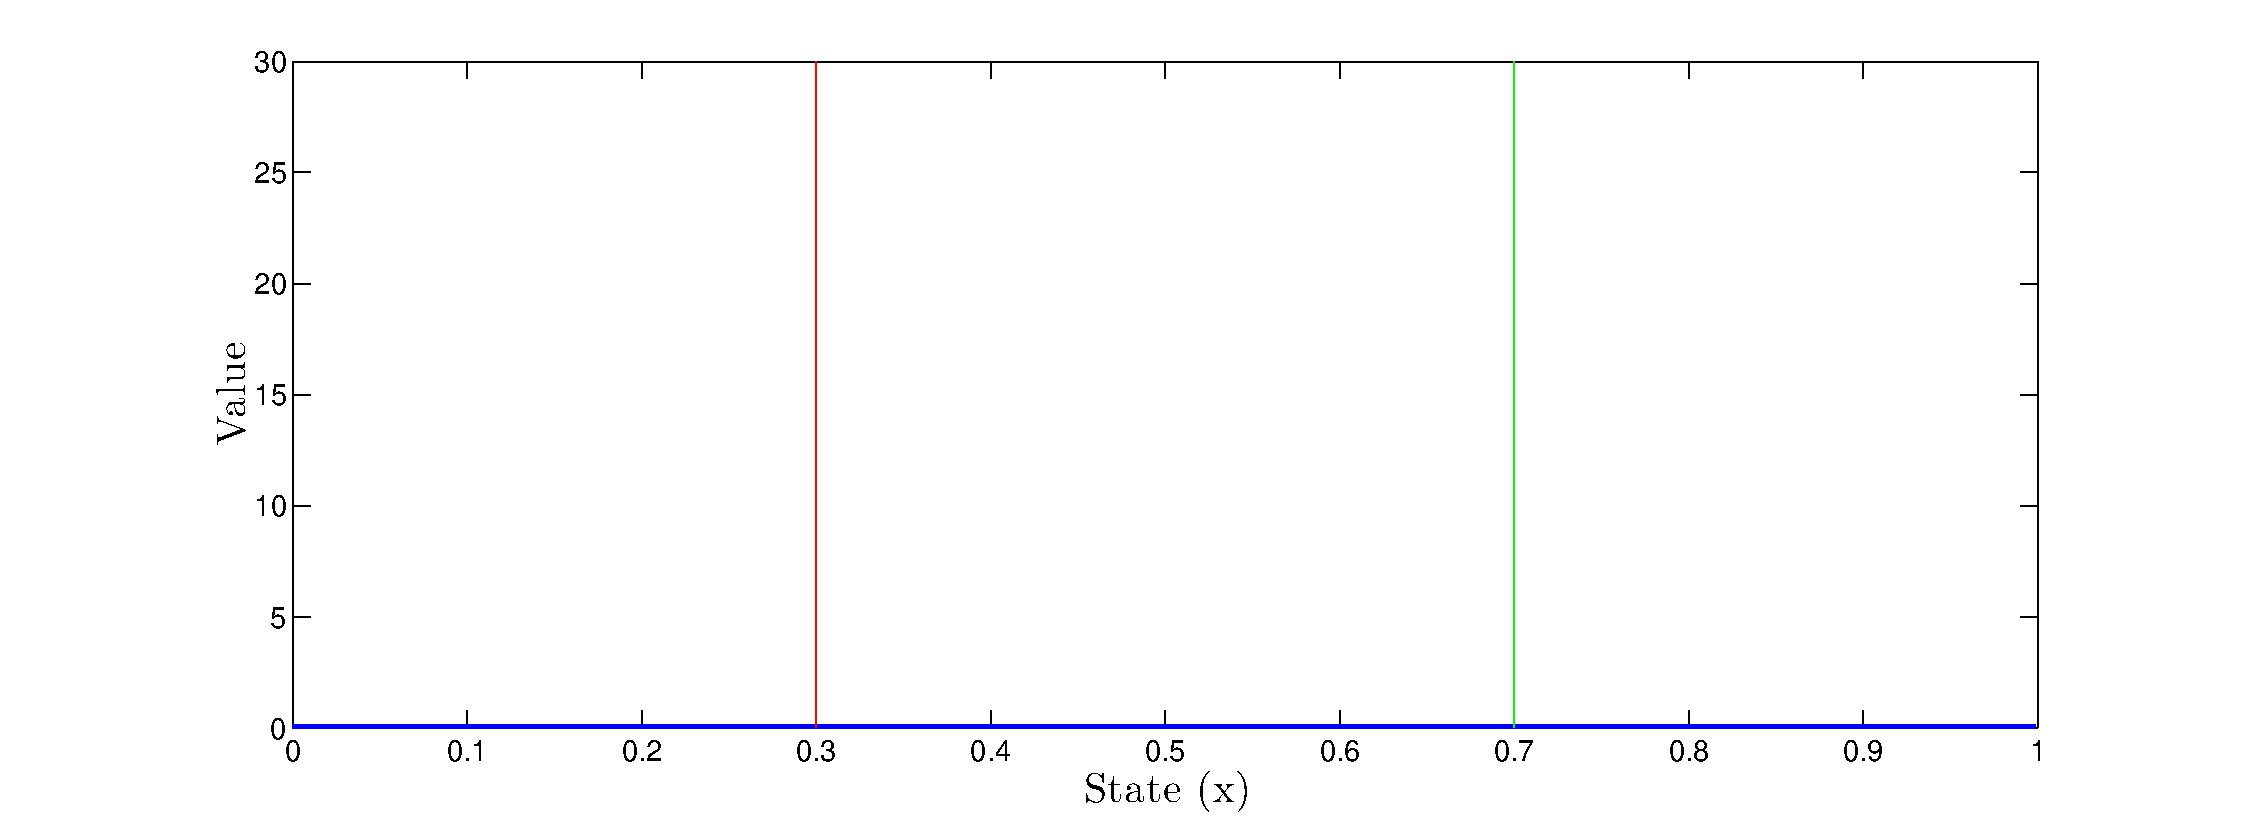
\includegraphics[width=260pt]{smp_sym.pdf}
\caption{Symmetric rewards.}
\label{fig:smpasmreward1}
\end{subfigure}

\begin{subfigure}[b]{0.5\textwidth}
\centering
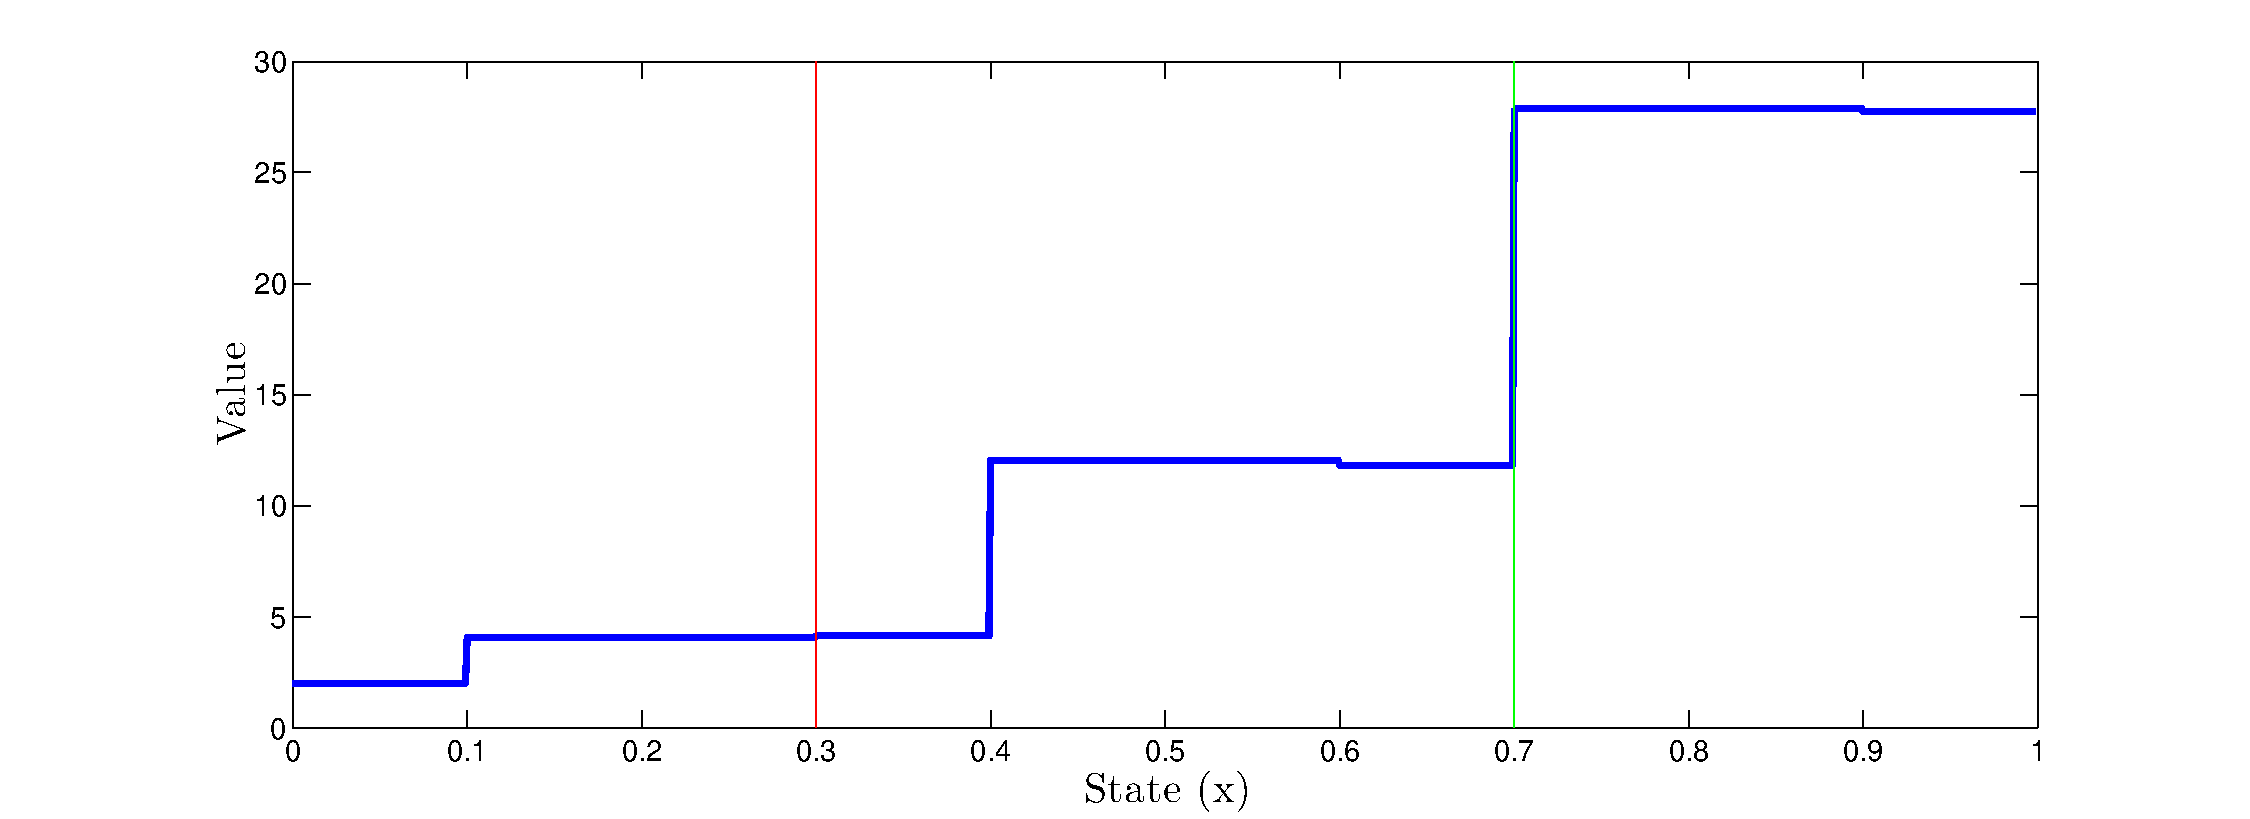
\includegraphics[width=260pt]{smp_asym.pdf}
\caption{Asymmetric rewards.}
\label{fig:smpasmreward2}
\end{subfigure}

%\vspace{-2mm}
\caption{The optimal value functions of the continuous stochastic matching 
            pennies game  for Player 1 at horizon 4 under (a) symmetric and (b) asymmetric reward 
            structures. Threshold values are set to $c = 0.3$
            and $d = 0.7$ and are highlighted in red and green, respectively. 
            The step size is $k = 0.3$.}
\label{fig:smpasmreward}
\end{figure}
%------------------------------------------------------------------------------

Figure~\eqref{fig:smpasmreward1} shows the results of the continuous
stochastic matching pennies game using the symmetric reward structure
given in Table~\ref{tab:smpsymreward}. The results show that the expected 
reward for Player 1 remains at zero over all 4 horizons, irrespective of the state \textit{x}. 
The symmetric reward structure clearly shows that both players achieve
the same expected reward in all regions \textit{r}. This in turn ensures that
both players are indifferent between their pure strategies. Hence, the expected reward 
for each player is zero in all regions. This result corresponds to the well known solution of the 
matching pennies game with symmetric rewards and serves as a proof of concept for 
our novel solution technique.

Figure~\eqref{fig:smpasmreward2} shows the effect of the asymmetric reward structure given in
Table~\ref{tab:smpasymreward}. The figure shows that Player 1 achieves the highest expected
reward in Region 3, followed by Region 2 and finally by Region 1. This corresponds
to the expected reward within each region of Table~\ref{tab:smpasymreward}. The results indicate 
that the Player 1 is no longer indifferent between its pure strategies in each region and may take short-term
losses to reach more favourable regions.

\subsection{Binary Option Stochastic Game}

Binary options are financial instruments which allow an investor to
bet on the outcome of a yes/no proposition. The proposition typically
relates to whether the price of a particular asset that underlies the option
will rise above or fall below a specified amount, known as the strike
price, $\kappa \in \mathbb{R}$. When the option reaches maturity the 
investor receives a fixed pay-off if their bet was correct and nothing otherwise.

\vspace{-1mm}

\subsubsection{Domain Description}

We analyse the valuation of a binary option as an extensive form
zero-sum game between a trader and the market. The aim of the trader
is to maximise their expected discounted pay-off at a fixed horizon $H$ 
through buying and selling options within an adversarial market. 
The problem has two state variables: the underlying market value of the asset
$v \in [0, 100]$ and the trader's inventory of options $i \in \mathbb{N}$.

At each time step the trader can execute one of three actions
$a_{trd} \in \left\{buy_{trd}, sell_{trd}, hold_{trd}\right\}$, where $buy_{trd}$ refers to a request to 
buy an option from the market, $sell_{trd}$ refers to a request to sell an option to
the market and $hold_{trd}$ is equivalent to taking no action. 
The market can execute one of two actions: $a_{mkt} \in \left\{sell_{mkt}, nsell_{mkt} \right\}$,
where $sell_{mkt}$ corresponds to selling an option to the trader and $nsell_{mkt}$ 
corresponds to not selling to the trader. 

The joint actions of the trader and market, $a_{trd}$ and 
$a_{mkt}$, respectively, affect both the underlying market value of the asset
and the trader's inventory. For the sake of simplicity we assume that
the market value may increase or decrease by fixed step sizes, 
$u \in \mathbb{R}$ for an increase and $d \in \mathbb{R}$ for a decrease.

The trader's option inventory dynamics are given by:

{\small 
\abovedisplayskip=0pt
\belowdisplayskip=0pt
\begin{align*}
& P(i' | v, i, a_{trd}, a_{mkt}) = \\
& \hspace{40pt} \delta \left[ i' - \begin{cases}
      (buy_{trd}) \wedge (sell_{mkt}) : & i + 1 \\ 
      (sell_{trd}) \wedge (i > 0) : & i - 1 \\
      otherwise: & i \\
    \end{cases} \right]
\end{align*}
}%

It should be noted that under this formulation the market will always
buy an option from the trader when the trader selects $sell_{trd}$. 
The market value changes according to:

{\small 
\abovedisplayskip=0pt
\belowdisplayskip=0pt
\begin{align*}
& P(v' | v, i, a_{trd}, a_{mkt}) = \\
& \hspace{40pt} \delta \left[ v' - \begin{cases}
      (buy_{trd}) \wedge (sell_{mkt})  : & v + u \\
       (sell_{trd}) \wedge (i > 0) : & v - d \\
      otherwise: & v
    \end{cases} \right]
\end{align*}
}%

Assuming that the strike price $\kappa \in [0, 100]$, the rewards obtained by the trader are given by:

{\small 
\abovedisplayskip=0pt
\belowdisplayskip=0pt
\begin{align*}
  R_{trader} = 
    \begin{cases}
      (sell_{trd}) \wedge (i > 0) \wedge (v > \kappa) : & 1 \\ 
      otherwise : & 0 \\
    \end{cases} \nonumber
\end{align*}
}%

The market's reward is simply the additive inverse of the trader's 
reward. Hence, the binary option game is zero-sum. 

\subsubsection{Results}

%%%%%%%%%%%%%%%%%%%%%%%%%%%%%%%%%
% Figure
\begin{figure}[h!]
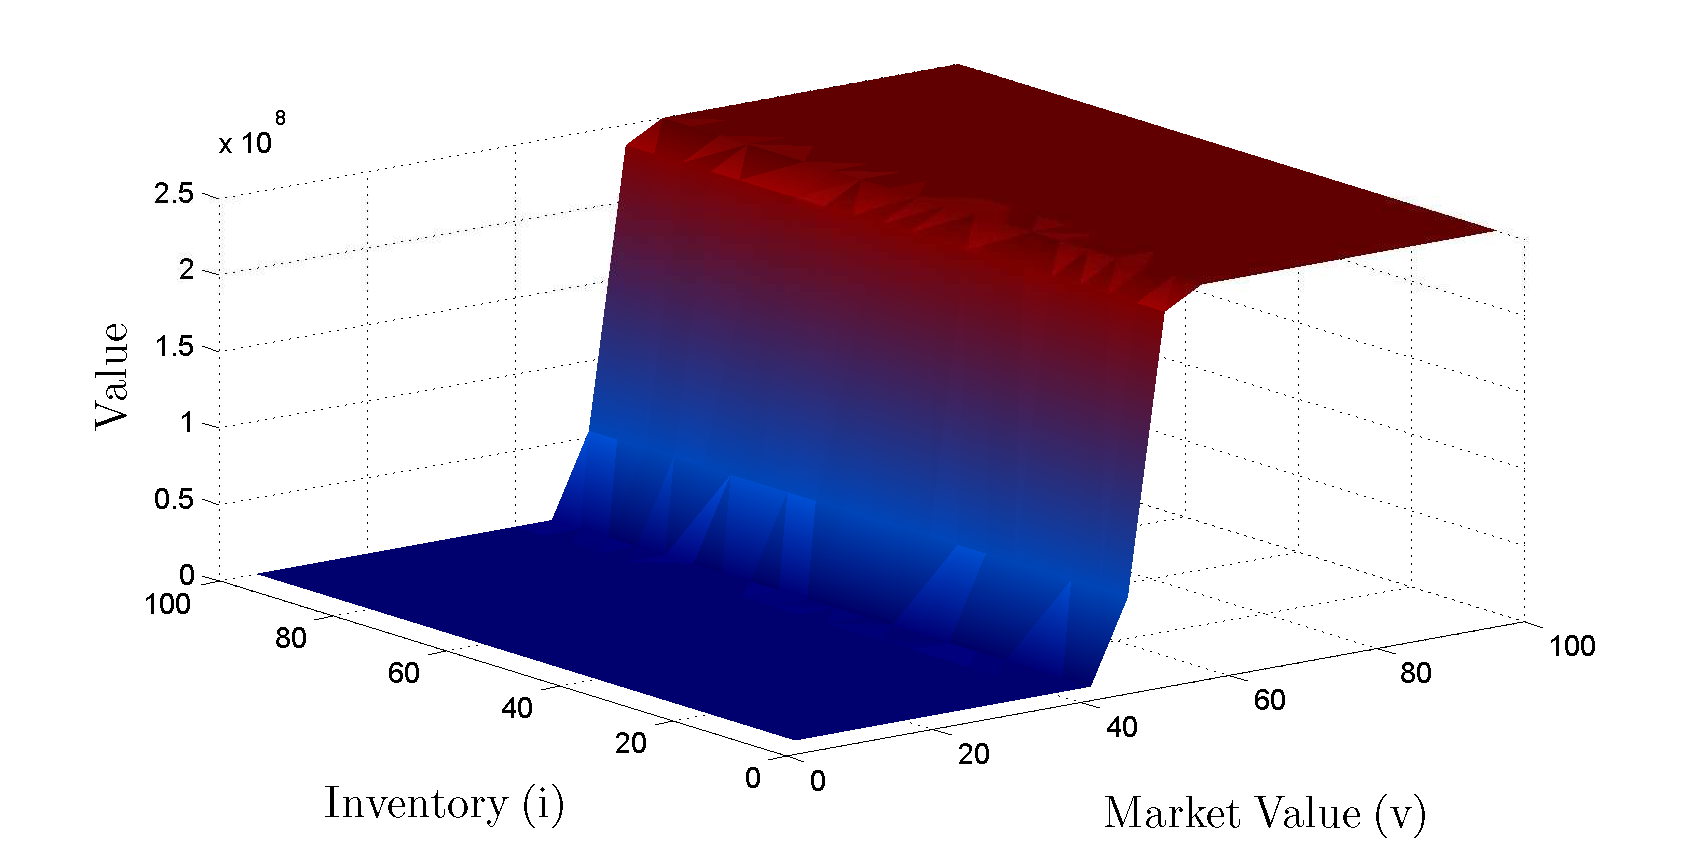
\includegraphics[width=250pt]{sbo.pdf}
%\vspace{-3mm}
\caption{The optimal value function of the binary option stochastic game for the trader at horizon 20. 
The strike price is set to $\kappa = 45.0$ and the increment and
decrement values are set to $u = 1.0$ and $d = 1.0$, respectively. Under the domain specification
the value function is invariant to the inventory $i$. }
\label{fig:binaryoptionvfunc}
\end{figure}
%%%%%%%%%%%%%%%%%%%%%%%%%%%%%%%

In Figure~\eqref{fig:binaryoptionvfunc} we show the optimal value function for the
binary option game at horizon 20. The strike price is set to $\kappa = 45.0$ and
the increment and decrement values, $u$ and $d$ are both set to 1.0. The
value function clearly shows that under this formulation the trader
achieves the most reward by selling options as soon $v > \kappa$.
Selling an option causes the underlying value to decrease. Once the value
falls beneath the strike price, the trader will buy options, which increases
the underlying value. This leads to the continual cycling of buying and selling 
of the option at values close to the strike price $\kappa$. In essence the trader 
behaves like a market maker in that they take both sides of the transaction at values near 
$\kappa$. We note that while Figure~\eqref{fig:binaryoptionvfunc} is invariant to the inventory
of options $i$, its inclusion is critical for the correct formalisation of the domain.

\subsection{Robust Energy Production}

The provision of energy resources is an integral component of any
economy. Energy providers must be able to produce energy in response
to changes in energy demand. In situations where demand exceeds supply,
an energy crisis may occur. In this paper we investigate energy 
production from the viewpoint of an energy provider responsible for 
supplying energy in an adversarial environment.

\subsubsection{Domain Description}

We define our energy production domain as an extensive form zero-sum
game between an energy provider and nature. The aim of the energy
provider is to maximise its expected discounted reward at a 
fixed horizon $H$ by changing production levels in response to changes in demand.
The domain has two state variables: the production level $p \in \mathbb{R}^{+}$ and the energy demand
$d \in \mathbb{R}^{+}$. 

At each time step the energy provider can execute one of two actions
$a_{prd} \in \left\{inc_{prd}, dec_{prd}\right\}$, where $inc_{prd}$ 
refers to increasing energy production and $dec_{prd}$ refers to decreasing
energy production. Nature can also execute one of two actions
$a_{nat} \in \left\{inc_{dem}, dec_{dem}\right\}$, where $inc_{dem}$ 
refers to increasing energy demand and $dec_{dem}$ refers to decreasing
energy demand. We specify the increase in the 
amount of energy produced or demanded by $prd_{u}, nat_{u} \in \mathbb{R}^{+}$ and a
corresponding decrease by $prd_{d}, nat_{d} \in \mathbb{R}^{+}$.

The joint actions of the energy provider and nature, $a_{prd}$ and
$a_{nat}$, respectively, affect the production level as follows:

{\small 
\abovedisplayskip=0pt
\belowdisplayskip=0pt
\begin{align*}
&P(p' | d, p, a_{prd}, a_{nat}) = \\
& \hspace{40pt} \delta \left[ p' - \begin{cases}
      (inc_{prd})  : & p + prd_{u} \\
       (dec_{prd}) \wedge (p > prd_{d}): & p - prd_{d} \\
      otherwise: & p
    \end{cases} \right] & \\    
\end{align*}
}%

The energy demand changes according to:
{\small 
\abovedisplayskip=15pt
\belowdisplayskip=0pt
\begin{align*}
&P(d' | d, p, a_{prd}, a_{nat}) = \\
& \hspace{40pt}\delta \left[ d' - \begin{cases}
      (inc_{dem})  : & d + nat_{u} \\
       (dec_{dem}) \wedge (d > nat_{d}) : & d - nat_{d} \\
      otherwise: & d
    \end{cases} \right] & \\    
\end{align*}
}%

The reward obtained by the energy provider are specified as:

{\small 
\abovedisplayskip=0pt
\belowdisplayskip=0pt
\begin{align*}
  R_{prd} = 
    \begin{cases}
      (p < d) : & -100 \\ 
      otherwise : & 0 \\ 
    \end{cases} \nonumber
\end{align*}
}%

We note that under this reward structure failure to meet energy demand
is heavily penalised, whereas meeting or even exceeding demand are
given the same reward. Nature's reward is simply the additive inverse 
of the energy provider's reward.

\subsubsection{Results}

%%%%%%%%%%%%%%%%%%%%%%%%%%%%%%%%%
% Figure
\begin{figure}[ht!]
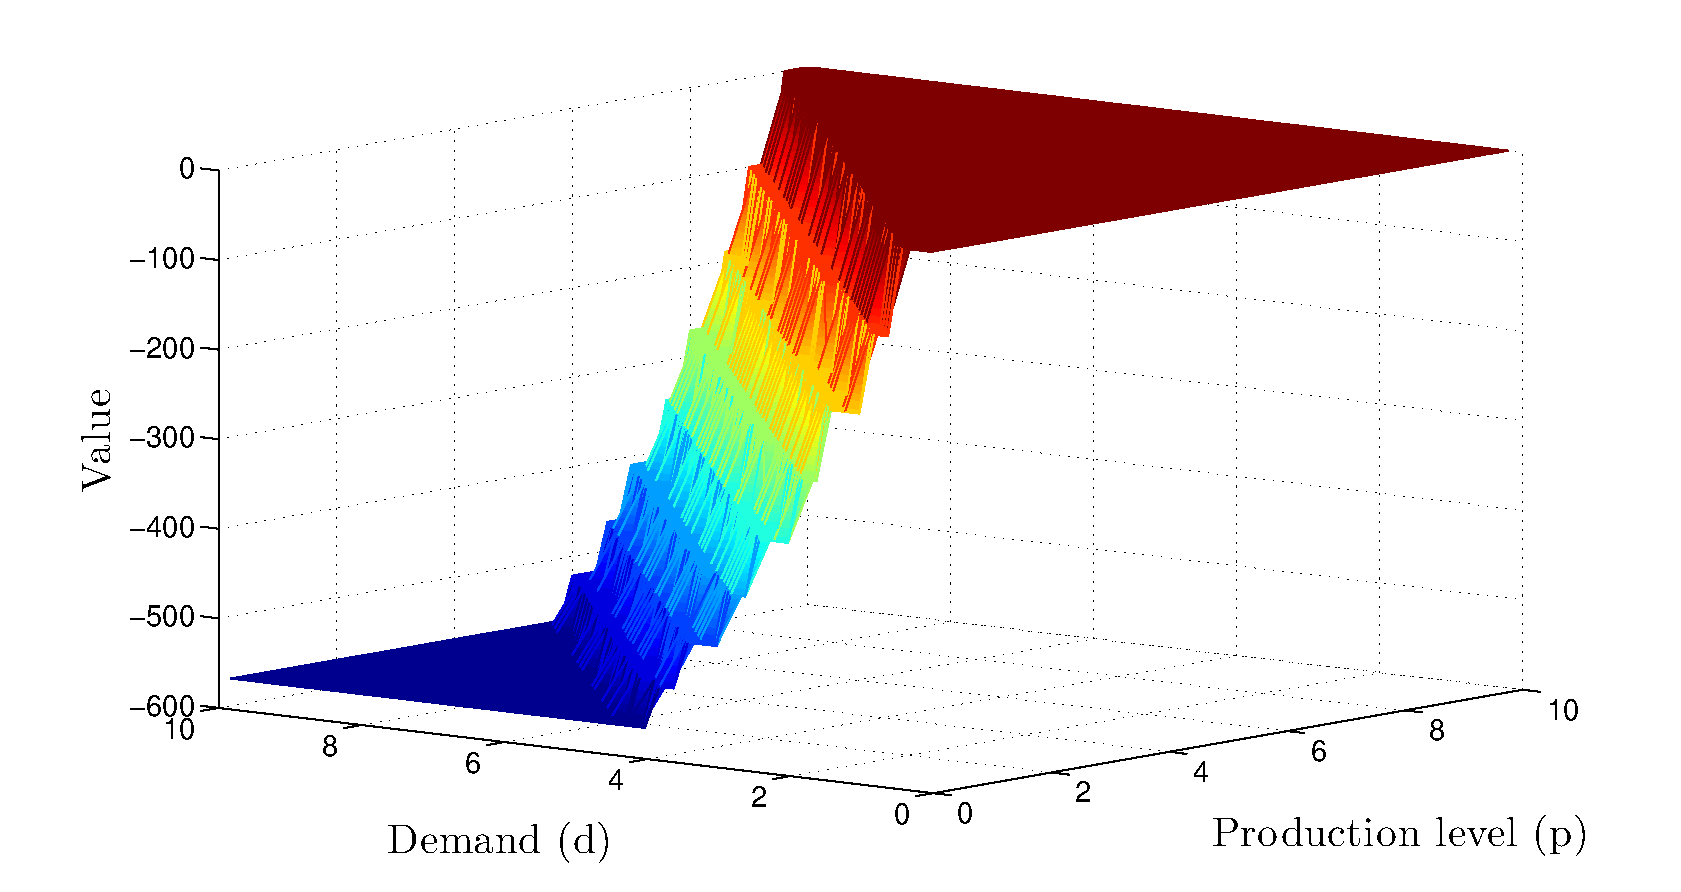
\includegraphics[width=250pt]{sep.pdf}
%\vspace{-3mm}
\caption{The optimal value function of  the robust energy production game for the producer at horizon 8. 
The production and demand increase and decrease variables were set to $prd_{u} = prd_{u} = 1.0$ and 
$nat_{u} = nat_{d} = 0.5$, respectively.}
\label{fig:sepvfunc}
\end{figure}
%%%%%%%%%%%%%%%%%%%%%%%%%%%%%%%%%

In Figure~\eqref{fig:sepvfunc} we show the optimal value function
for the robust energy production game at horizon 8. The production and demand 
increase and decrease variables were set to $prd_{u} = prd_{u} = 1.0$ and $nat_{u} = nat_{d} = 0.5$, respectively.
The value function shows that the energy provider achieves the highest value when the energy provided
meets or exceeds demand. The value function is lowest when the demand exceeds supply, which is in accordance
with the reward structure. The value function clearly decreases in a step-wise manner from the point 
where the production level meets demand, indicating that production levels just beneath demand have a higher value than
those well below demand.

\section{Related Work}
\label{sec:relatedwork}

Solutions to stochastic games have been proposed from within both
game theory and reinforcement learning. The first algorithm, game theoretic or otherwise, for 
finding a solution to a stochastic game was given by Shapley \cite{Shapley_PotNAoS_1953}.
The algorithm repeatedly calculates a value function $V(s)$ over discrete states
which converges to an optimal value function $V^{*}(s)$, which represents
the expected discounted future reward if both players in the game followed
the game's Nash equilibrium. Shapley's algorithm is in essence an 
extension of the value iteration algorithm to stochastic games. A reinforcement 
learning based solution to stochastic games was first introduced by 
Littman \cite{Littman_ICML_1994}. Littman's algorithm, Minimax-Q,
extends the traditional Q-learning algorithm for MDPs to 
zero-sum discrete stochastic games. The algorithm converges to the 
stochastic game's equilibrium solution. Hu and Wellman \cite{Hu_ICML_1998}
extended Minimax-Q to general-sum games and proved that it converges
to a Nash equilibrium under certain restrictive conditions. Although
both reinforcement learning based algorithms are able to calculate 
equilibrium solutions they are limited to discrete state formulations of
stochastic games. In this paper we calculate exact solutions to 
continuous state formulations of stochastic games, under certain restrictions.
The Dec-MDP \cite{Bernstein_MoOR_2002} framework allows
for decentralised control within continuous state spaces but is limited
to general-sum systems. In this paper we provide the first 
known exact closed-form solution to a subclass of continuous state zero-sum 
stochastic games defined by a piecewise constant reward and piecewise linear transition.

Several techniques have been put forward to tackle continuous state
spaces in MDPs. Li and Littman \cite{Li_AAAI_2005} describe a method
to approximate intermediate piecewise linear value functions by piecewise
constant functions, which results in approximate solutions to continuous
state MDPs. Furthermore, Li and Littman only allow for rectilinearly aligned 
constraints in their reward and transition functions, not arbitrary linear constraints,
and cannot handle general linear transition models without approximating.  
Our SDP method provides exact solutions without these restrictions, which
makes SDP strictly more general. Finally, Li and Littman did not consider 
game-theoretic extensions of their work or the parameterised optimisation 
problem that these extensions entail.

Symbolic dynamic programming techniques have been previously used to calculate
exact solutions to single agent MDPs with both continuous state and actions
in a variety of non-game theoretic domains \cite{Sanner_UAI_2011,Zamani_AAAI_2012}.
In this paper we present the first application of SDP to stochastic games
with concurrently acting agents.

%----------------------------------------------------------------------------
%The use of reinforcement learning methods to solve stochastic games
%was introduced by Littman \cite{Littman_ICML_1994}. Under Littman's
%formulation optimal policies can be calculated for discrete state zero-sum 
%stochastic games using an algorithm akin to Q-learning. Hu \cite{Hu_ICML_1998}
%extended Littman's framework into the general-sum case. Whilst both
%approaches provide optimal policies for stochastic games under zero-sum
%and general sum settings, they are limited to discrete state formulations. 
%
%A lazy approximation technique for MDPs which imposes similar restrictions on the
%form of the reward and transition functions was introduced by Li \cite{Li_AAAI_2005}
%and allows for the calculation of approximate solutions. Our approach using
%symbolic dynamic programming calculates exact solutions in game theoretic
%settings. 






\section{Conclusions}
\label{sec:conclusion}

% Contributions
% Place work in wider context
% Future research directions

We have characterised a subclass of zero-sum continuous stochastic
games that can be solved exactly via parameterised linear optimisation.
We have also presented a novel symbolic dynamic programming 
algorithm that can be used to calculated exact solutions to this subclass
of stochastic games for arbitrary horizons. The algorithm
was used to calculate the first known exact solutions to a variety of 
experimental continuous domains.

%-----------------------------------------------------------------------------
%In this paper, we have introduced a novel symbolic dynamic programming
%technique to calculate exact solutions to a subclass of continuous state
%zero-sum stochastic games. Our key contributions are two-fold: we characterise
%a subclass of continuous stochastic games that can be solved 
%optimally in closed-form and we also prove that this solution remains
%closed-form for arbitrary horizons. This paper also represents the first
%extension of symbolic dynamic programming into game-theoretic domains.
%
%We believe that this work is the first to provide optimal closed-form
%solutions to continuous stochastic games with continuous state, 
%piecewise linear dynamics and piecewise constant reward. Furthermore,
%we assert that our experimental results are the first to provide
%exact solutions to their domains.

There are a number of avenues for future research. Firstly, it is important
to examine more general representations of the reward and transition functions while
still guaranteeing exact solutions. Another direction of research lies within
improving the scalability of the algorithm by using techniques such as 
bounded error compression for XADDs \cite{Vianna_UAI_2013} or lazy 
approximation of value functions as piecewise linear XADDs \cite{Li_AAAI_2005}. 
Search based approaches such as RTDP \cite{Barto_AI_1995} and HAO* \cite{Meuleau_JoAIR_2009}
are also readily adaptable to SDP. These extensions may then be used to 
model more complex financial and economic domains. Finally, SDP can be
used to calculate exact solutions to general sum stochastic games. The advances
made by this work open up a number of potential novel research paths
that we believe may help make progress in solving game theoretic domains
with continuous state.


\newpage

% Hacky way to implement the Reference heading. 
% UAI requires an unnumbered third level heading
\subsubsection*{References}
\begingroup
\renewcommand{\section}[2]{}%
\bibliographystyle{authordate1}
\bibliography{uai2014}
\endgroup

\end{document}
